\chapter{SDN中LDoS方案设计}
\label{cha:design}
本章的主要内容为LDoS防御方案的设计。首先,对LDoS的特征进行分析,找到防御LDoS的关键点点。然后,根据防御LDoS的要点,结合SDN的优势设计了SDN中防御LDoS的两种方案。最后,对两种方案的设计思想和实现方案进行探索和分析。本文是基于SDN中最经典的OpenFlow协议完成设计的。

\section{SDN中LDoS防御的关键点分析}
\label{chap4:keyanalysis}
前文已经对LDoS攻击的攻击形式有了说明,本文首先分析单一攻击源的LDoS攻击实现的关键点并找到合适的防御机制。LDoS攻击的核心思想就是通过周期性的引发TCP流丢包,触发TCP拥塞控制机制或者超时重传机制降低TCP流的吞吐量,最后达到以极低的流量使TCP流异常的目标。因此,本文防御LDoS有两种核心思想,第一种是采取措施使TCP流不丢包,第二种是找到并限制攻击源。

第一种思想是采取措施使得TCP流不丢包。通过前文可知,TCP流的丢包是由于LDoS的速率太高拥塞队列导致的。所以,只要交换机保护TCP流的最低通信需求,则TCP不会因为收不到任何包而进入超时重传状态。在SDN网络中,带宽保障可以通过SDN中特有的meter规则去实现,使用meter规则限制其他流的最高速率从而给TCP流提供有最低速率保障,则LDoS无法通过拥塞队列强迫TCP流完全丢包。从而达到防御LDoS攻击的效果。但是,这样的做法在LDoS攻击的突发到达的时候,速率依然会降得很低,而拥塞窗口也会相应的减小,因此,这种思想只能减轻攻击所造成的危害,但是不能完全消除LDoS攻击对TCP流的影响。

第二种思想是找到并且限制攻击源。在SDN网络中,所有的数据转发都是由流表规则匹配完成的,因此,在SDN中可以实现流级别的数据分析。由于LDoS攻击拥塞了某个交换机的队列才能实现攻击,因此,可以在交换机的端口处检测LDoS是否存在。LDoS攻击作为一个周期性的“方波”是能够由周期性来确认的,因此,在端口处只要能够确认有周期性的吞吐量变化,就能够确认攻击,再之后通过流级别的分析判断攻击流,最后,再对判断出来的攻击流的攻击源进行限制。使用这种思想来防御LDoS攻击就能够完全消除LDoS攻击流对TCP流的影响,但是,在攻击开始的时候TCP流会受到一定的影响,可能会出现部分TCP流进入超时重传状态,影响吞吐量。

\section{SDN中基于带宽保障的LDoS防御方案}
\label{chap4:bandguatee}

保证TCP流不进入超时重传状态,防御方案必须保证TCP流无论在什么情况下都不能丢包,结合SDN的特性,该方案结合OpenFlow的Meter规则来实现,可以最大程度利用SDN网络可以自由制定网络规则的特性。

首先,分析Meter规则是如何在SDN中运行的,才能制定Meter规则防御LDoS攻击。Meter规则允许SDN实现各种各样的服务质量(Quality of Service,QoS)配置,其中就包括了速率限制。Meter规则能够直接与SDN中的流表规则绑定,这个Meter规则可以测量和控制所有与之绑定的流表规则的聚合速率,因此,Meter规则可以用来限制除TCP流以外的所有流聚合的速率。

\begin{table}[htbp]
	\centering  % 显示位置为中间
	\caption{Meter规则}  % 表格标题mn9GFFFFFFFFFFFFFFFFFFFFFFFFFFFFFFFFFFFFFFFFFFFFFFFFFFFFFFFFFFFF
	\label{table:meter}  % 用于索引表格的标签
	%字母的个数对应列数,|代表分割线
	% l代表左对齐,c代表居中,r代表右对齐
	\begin{tabular}{|c|c|c|}  
		\hline  % 表格的横线
        Meter Identifier & Meter Bands& Counters \\  % 表格中的内容,用&分开,\\表示下一行
        \hline
		
	\end{tabular}
\end{table}

表\ref{table:meter}为SDN的Meter规则的主要内容。Meter Identifier是一个32比特的无符号整数,它能够用于唯一标识一个Meter规则。counters是统计与meter绑定的流表规则的统计相关数据,随时更新。其中,最重要的是Meter Bands,它是Meter规则控制和限制绑定聚合流的速率和处理包方式的的部分。需要注意的是,每个Meter规则可以匹配多个Meter Band。表\ref{table:meterbands}为一个Meter Band部分,它由五个部分组成,首先是Band Type部分,这直接定义了速率超过限定速率以后,后面的包是如何处理的。此处有两种选项:一种为\emph{drop},这样它该Meter规则就可以被用来限制速率;一种为\emph{dscp remark},这样就能增加数据包IP头中DSCP字段的丢弃优先级,可用于定义不同级别的服务。第二个参数是Meter规则限制的速率,它定义Meter规则最低适用的速率,若是速率高于该参数的数据包则需要根据Meter规则进行处理。Counters表示被该Meter Band处理的包的统计数据。Burst参数是本文需要调的一个重要参数,该参数定义了Meter Band的粒度。Type specific arguments表示band types有特殊的参数。

\begin{table}[htbp]
	\centering  % 显示位置为中间
	\caption{Meter Band}  % 表格标题
	\label{table:meterbands}  % 用于索引表格的标签
	%字母的个数对应列数,|代表分割线
	% l代表左对齐,c代表居中,r代表右对齐
	\begin{tabular}{|c|c|c|c|c|}  
		\hline  % 表格的横线
        Band Type & Rate & Burst & Counters & Type specific arguments \\  % 表格中的内容,用&分开,\\表示下一行
        \hline
		
	\end{tabular}
\end{table}

此方案使用Meter规则来实现对非TCP流的速率限制,这样就能够对LDoS攻击进行限制。但是,由于LDoS攻击具有一定的特殊性,普通配置Meter规则无法限制LDoS攻击,需要特殊的配置。首先,由于LDoS攻击会拥塞某个端口的队列,所以,对于每个激活的端口,都应当配置一个相应的Meter规则进行限制,对于从端口处发送非TCP数据的流表规则需要与该端口的Meter规则进行绑定,受该Meter规则的束缚。接下来,Meter规则的粒度也需要特殊的配置,默认的状态下,Meter规则是以1秒作为统计单位进行速率限制的,由于LDoS攻击的平均速率并不能满足Meter规则限制的需求,因此Meter Band设置的Burst参数需要重新配置。接下来,需要设置Rate参数的大小来限制非TCP聚合流的速率,设置的参数数值大了会影响其他正常流的速率,设置的值过小会使TCP流的窗口降至极小的程度,达不到限制LDoS攻击的效果。因此,该参数对窗口大小的影响非常重要。


基于带宽保障的LDoS防御方案可以分为两个阶段完成。流程图如\ref{fig:meter-solution}所示。防御方案的第一阶段为预配置Meter规则阶段,控制器首先会检测所有激活端口,并给每个端口分配一个Meter规则,Meter规则需要调节Burst参数使得粒度在RTT级别大小,这样才能够有效的限制LDoS攻击的速率。其次,设置合理的Rate参数保证TCP流不进入超时重传机制的同时使滑动窗口不至于变得太小。设置Band Type为drop,这样就丢弃所有超速的包,可以保障了TCP流有一定的带宽可以使用。防御方案的第二个阶段为流处理阶段,有一个流进入交换机,则需要对该流进行区分处理。若是该流为TCP流,则该TCP流的流表不需要绑定任何Meter规则,这样它就不会被Meter规则所束缚,可以按照TCP拥塞控制的机制进行速率的控制。若是该流不是TCP流,则需要绑定Meter规则以保证该流不会对TCP流造成损害,特别是当该流为LDoS攻击流的时候,由于速率被控制,队列不会被该流所拥塞而造成TCP流丢包,TCP流就不会进入超时重传状态。

\begin{figure}
    \centering
    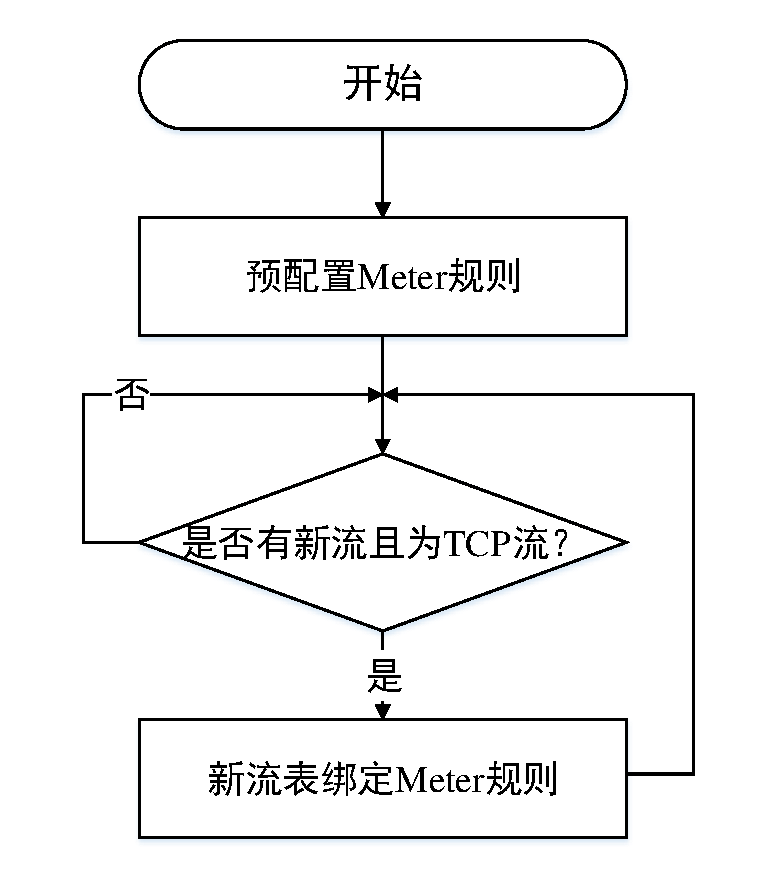
\includegraphics[scale=1]{meter-solution}
    \caption{基于带宽保障的LDoS防御方案流程图}
    \label{fig:meter-solution}
\end{figure}


\section{SDN中基于动态周期性检测的LDoS防御方案}
\label{chap4:SoftGuard}
为了保证SDN网络的正常传输,基于动态周期性检测的方案也被

\begin{table}[htbp]
	\centering  % 显示位置为中间
	\caption{流表规则中的主要内容}  % 表格标题
	\label{table:flowrule}  % 用于索引表格的标签
	%字母的个数对应列数,|代表分割线
	% l代表左对齐,c代表居中,r代表右对齐
	\begin{tabular}{|c|c|c|c|c|c|c|c|}  
		\hline  % 表格的横线
        Match & Fields & Priority & Counters & Instructions & Timeouts & Cookie & Flags \\  % 表格中的内容,用&分开,\\表示下一行
        \hline
		
	\end{tabular}
\end{table}

